% Target: 35 pages
% Current: 3

\chapter{Adapters in Machine Translation}
\label{chap:adaptmt}
This chapter aims to study the impact of pre-trained models when fine-tuning machine translation models with adapters. Specifically, we are interested in understanding the contribution of good representation in the pre-trained language model to the adapters during fine-tuning. Furthermore, we are also interested in understanding the capability of adapters to perform with artificially degraded pre-trained models. We propose to use transformer-based architecture such as BERT (pre-trained or trained from scratch) for both the encoder and decoder components while using adapters for fine-tuning. To be more specific, we divide the experiments into four different pre-trained model setups:
\begin{itemize}
    \item Use BERT weights\footnote{We use publicly available BERT weights from Huggingface hub \url{https://huggingface.co}} as the pre-trained weights (\texttt{Pre-trained BERT}). We use this model as the baseline for our experiments in this chapter.
    \item Use randomly initialised BERT models and pre-train the models with MLM objective on IWSLT and WMT data (\texttt{Pre-trained Transformer}). This setup is used to understand the impact of different data volumes and domains on the quality of the pre-trained models that will be fine-tuned with adapters in the later phase.
    \item Use the pre-trained BERT model where the weights within the same layer are shuffled (\texttt{Pre-trained shuffled}). We use this setup to understand whether the adapters can capture important features from the original BERT weights and restore the performance even though the weights are no longer in the original position.
    \item Use randomly initialised BERT models with no pre-training (\texttt{Pre-trained random}). We use this setup as a complement of \texttt{Pre-trained shuffled} experiments to understand the impact of pre-trained models that contain relatively inferior knowledge than the original BERT model on the adapters when fine-tuned in the MT task.
\end{itemize}

\section{Experiments Setup}
\subsection{Language Model}
\label{ssec:langmodel}
\subsubsection{Dataset}
\label{ssec:langmodeldataset}
From \cite{devlin2018bert}, we understand that BERT was trained with billions of words from various sources and domains. However, we do not fully understand the proper condition to stop adding more sentences to the pre-training data so that we can reduce the hours of training the model. Additionally, we do not know the impact of combining different domains in the pre-training data on the final performance of the model. For those reasons, we are reducing the scope of the pre-training data by restricting the creation of pre-training data only from machine translation datasets in two different domains and constructing the pre-trained models with different sizes of data. We use WMT and IWSLT for the experiment as WMT and IWSLT contain different domains, and WMT has a significantly larger volume and longer sentences. Specifically, we construct three different datasets with different volumes:
\begin{enumerate}
    \item A standalone IWSLT.
    \item A combination of IWSLT and WMT data with a total of 500k sentences. We add the randomly sampled WMT data on top of IWSLT to increase the volume of our pre-training data. We should also note that the domain of WMT differs from the IWSLT, and we only test the models on the IWSLT test set. The WMT data can thus lead to worse translation performance due to domain mismatch.
    \item A combination of IWSLT and WMT data with 2 million sentences. The same as (2) but with larger volumes.
\end{enumerate}

Datasets (2) and (3) were constructed with a simple approach by using all training data from IWSLT, randomly selecting sentences from the WMT dataset, and combining them until we met the required number of sentences mentioned in the previous paragraph.

The objective of the 500k dataset is to see the model's performance when more data from a general domain (WMT19) is included, but the distribution still favours the target domain (IWSLT14). This could help understand whether randomly sampling data from the general domain and incorporating them while keeping the target domain as the majority in the training set can help the final performance for either language model pre-training or direct machine translation. The 2 million dataset has a similar objective, but now the distribution differs from the standalone IWSLT and 500k datasets. The dataset is now dominated by the general domain and contains various topics that may or may not be related to the target domain. From this distribution shift, we would like to understand the impact on the model and the final performance.
We understand it would be preferable to have more granularity by including more sizes, such as more than 2 million sentences, to understand the model's actual limit better when more sentences are added. However, due to time and resource considerations, we limit the experiments in this thesis to only the combination mentioned above.
% \hl{The objective of the 500k dataset is to see the model's performance when more data from a general domain (WMT19) is included, but the distribution still favours the target domain (IWSLT14). This could help understand whether randomly sampling data from the general domain and incorporating them while keeping the target domain as the majority in the training set can help the final performance for either language model pre-training or direct machine translation. The 2 million dataset has a similar objective, but now the distribution differs from the standalone IWSLT and 500k datasets. The dataset is now dominated by the general domain and contains various topics that may or may not be related to the target domain. From this distribution shift, we would like to understand the impact on the model and the final performance.
% We understand it would be preferable to have more granularity by including more sizes, such as more than 2 million sentences, to understand the model's actual limit better when more sentences are added. However, due to time and resource considerations, we limit the experiments in this thesis to only the combination mentioned above.}

\begin{table}[]
    \centering
    \begin{tabular}{@{}|l|l|l|l|@{}}
        \toprule
        \multicolumn{1}{|c|}{\textbf{Dataset}}                                                          &
        \multicolumn{1}{c|}{\textbf{Initial Weights}}                                                   &
        \multicolumn{1}{c|}{\textbf{\begin{tabular}[c]{@{}c@{}}Used for \\ pre-training?\end{tabular}}} &
        \multicolumn{1}{c|}{\textbf{\begin{tabular}[c]{@{}c@{}}Used for \\ fine-tuning?\end{tabular}}}                                 \\ \midrule
        \multirow{2}{*}{Standalone IWSLT}                                                               & Pre-trained BERT & No  & Yes \\ \cmidrule(l){2-4}
                                                                                                        & Random BERT      & Yes & Yes \\ \midrule
        IWSLT + WMT 500k                                                                                & Random BERT      & Yes & No  \\ \midrule
        IWSLT + WMT 2m                                                                                  & Random BERT      & Yes & No  \\ \bottomrule
    \end{tabular}
    \caption[IWSLT and WMT data usages with respect to the weights initialization.]{The initial weights represent the weights used on both the encoder and decoder. Pre-trained BERT refers to the pre-trained models that use BERT. Random BERT models use BERT configuration but not the weights. Therefore, contrary to the Pre-trained BERT, Random BERT models undergo a pre-training process before fine-tuning. The pre-trained and fine-tuned columns represent the boolean value to mark whether the models initialized with the targeted weights are pre-trained or fine-tuned with the respective data. For example, Huggingface BERT weights are not pre-trained with IWSLT but use IWSLT for fine-tuning.}
    \label{tab:mixeddataset}
\end{table}

To illustrate how the datasets are used in the experiments, we refer to \cref{tab:mixeddataset}. We can see that datasets other than standalone IWSLT are used only for pre-training. The IWSLT is always used for fine-tuning, and depending on the initial weights, we also use it as pre-training.

\subsubsection{Model}
To pre-train the model, we follow the work of \cite{devlin2018bert} by using the Masked Language Model (MLM) objective. In every sentence, some words will be masked, and the model has to predict the original words. A complete illustration can be found in \cref{img:mlmobj}.

\begin{figure}[h]
    {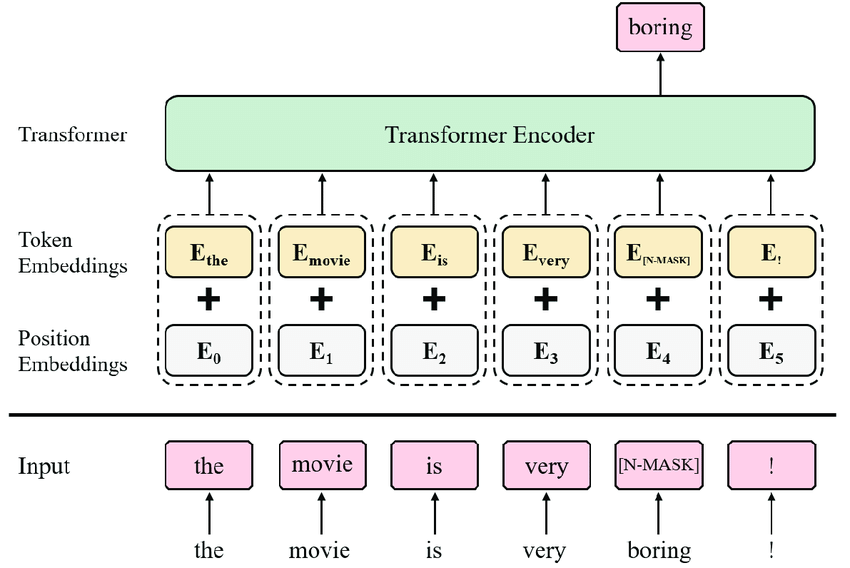
\includegraphics[width=0.85\textwidth]{img/mlm_obj.png}}
    \centering
    \caption{Illustration of the MLM objective during the pre-training. The illustration is reprinted from \cite{Park2019SelfSupervisedCD}.}
    \label{img:mlmobj}
\end{figure}

The MLM is introduced as an alternative objective to the auto-regressive language model. The auto-regressive objective is inherently different from the MLM. In auto-regressive, the models have to predict the word at step $t$, and they only have the ability to look at the previous words ($t-1...0$) as the context. Auto-regressive is used in a couple of works such as GPT models \citewithpar{brown2020language,ratford2019language,radford2018improving} for pre-training. One of the advantages of using the MLM compared to the auto-regressive is that we can exploit the bidirectional context rather than only predicting the words from left to right.

We use the default BERT configuration from Huggingface to construct the model. The complete list of hyperparameters for the model and the optimizer can be found in \cref{tab:hyp}.

\begin{table}[]
    \begin{tabular}{@{}lccc@{}}
        \toprule
        \textbf{Name}                   & \textbf{En} & \textbf{De} & \textbf{Description}                                                                         \\ \midrule
        vocab\_size                     & 30522       & 31102       & \begin{tabular}[c]{@{}c@{}}Vocabulary size of the\\ BERT model\end{tabular}                  \\ \midrule
        hidden\_size                    & 768         & 768         & \begin{tabular}[c]{@{}c@{}}Dimensionality for each\\ of the layers\end{tabular}              \\ \midrule
        num\_hidden\_layers             & 12          & 12          & \begin{tabular}[c]{@{}c@{}}Number of hidden layers\\ in the transformer\end{tabular}         \\ \midrule
        num\_attention\_heads           & 12          & 12          & \begin{tabular}[c]{@{}c@{}}Number of attention heads for\\ each attention layer\end{tabular} \\ \midrule
        intermediate\_size              & 3072        & 3072        & \begin{tabular}[c]{@{}c@{}}Dimensionality of the\\ feed-forward layer\end{tabular}           \\ \midrule
        hidden\_act                     & gelu        & gelu        & \begin{tabular}[c]{@{}c@{}}The activation function\\ within the layer\end{tabular}           \\ \midrule
        learning\_rate                  & 0.0005      & 0.0005      & \begin{tabular}[c]{@{}c@{}}Learning rate used\\ for the experiments\end{tabular}             \\ \midrule
        optimizer                       & adam        & adam        & \begin{tabular}[c]{@{}c@{}}Model optimizer\end{tabular}                                      \\ \midrule
        batch\_size                     & 64          & 64          & \begin{tabular}[c]{@{}c@{}}Batch size used\\ for the experiments\end{tabular}                \\ \midrule
        hidden\_dropout\_prob           &
        0.1                             &
        0.1                             &
        \begin{tabular}[c]{@{}c@{}}The dropout probability\\ for all fully connected layers in\\ the embeddings, encoder,\\ and pooler\end{tabular}                \\ \midrule
        attention\_probs\_dropout\_prob &
        0.1                             &
        0.1                             &
        \begin{tabular}[c]{@{}c@{}}The dropout ratio for the\\ attention probabilities\end{tabular}                                                                \\ \bottomrule
    \end{tabular}
    \caption[Transformer BERT hyperparameters for English and German.]{Transformer BERT hyperparameters for English (based on \texttt{bert-base-uncased}) and German (based on \texttt{bert-base-german-dbmdz-uncased}).}
    \label{tab:hyp}
\end{table}

We train the model until convergence with a maximum of 500 epochs. \hl{We limit the experiments to 500 epochs as we refer to one of our experiments, where we use BERT as the pre-training model and fine-tune it with adapters. It achieves a considerably good performance and converged in less than 500 epochs. We consider this model as our baseline in terms of both speed of training and evaluation score (BLEU). Due to this reason, we consider the speed of training or fine-tuning as one of the main factors for the experiments. We would like to see the performance of various models in both the speed as well as the final evaluation score.}
We define convergence by training for at least one day, with the validation loss no longer improving. We train the models in the MetaCentrum cluster with a specific configuration where the running jobs will be automatically killed after 24 hours. The loss usually starts to converge in less than 24 hours, but in some cases, we still see some models that are not yet converged. In this case, we continue the training by running another job process and loading the last checkpoint. On the other hand, if the loss starts to diverge before 24 hours or 500 epochs, we stop the training manually and select the checkpoint with the lowest loss score. Each language may end up converging in a different number of steps.

\subsection{Machine Translation}
\subsubsection{Dataset}
In machine translation experiments, there are several scenarios in which we use both WMT and IWSLT datasets. The IWSLT dataset is mainly used to fine-tune and evaluate the final model. The WMT, on the other hand, will be combined with IWSLT for training the baseline models. We use three different datasets for the experiments similar to the language model setup: IWSLT standalone, IWSLT + WMT (500k), IWSLT + WMT (2 million). To be more specific, we use the IWSLT standalone dataset for training, evaluation, and testing. The remaining data setups are used only for training, and we limit ourselves to the IWSLT data for evaluation and testing.

\subsubsection{Model}
We use the seq2seq architecture by \cite{vaswani2017attention}. The seq2seq architecture contains two components, the encoder and the decoder. We can refer to \cref{ssec:transformer} for further details on the architecture. The encoder and decoder use the same model and hyperparameters as described in \cref{ssec:langmodel}. The only difference from the original language model is on the decoder side. On the encoder side, we only use the self-attention layers to gather some context from the neighbours within the same layer. On the other hand, the decoder requires further context to generate its outputs by including the vector representation from the encoder as additional features. For this reason, an extra component named \texttt{cross\_attention} layer is introduced in the decoder, and it is trained from scratch in all experiments.

\section{Experiments Results}
This section discusses the results obtained for machine translation. First, in \cref{ssec:adaptcomp}, we conduct the comparative study of using adapters in different pre-trained scenarios. Second, in \cref{ssec:randshuff}, we perform a study by replacing the BERT model with a different BERT version where the weights are shuffled. We continue the experiments using pre-trained models with completely random weights and no pre-training. Finally, in \cref{ssec:randpre}, we perform experiments comparing the performance of the randomly set weights pre-trained model that is fine-tuned with adapters with the baseline models as well as models that are pre-trained with the combination of WMT and IWSLT.

\subsection{Adapters Comparison}
\label{ssec:adaptcomp}
\subsubsection{Experiment Setup and Motivation}
In this section, we conduct experiments to understand the contribution of adapt\-ers by comparing trained and fine-tuned models with different sizes of datasets. The definition of the dataset is the same as have already explained in the previous section. The dataset is used for two different purposes:
\begin{itemize}
    \item Used to train the BERT-style language model from scratch, separated for source and target languages.
    \item Used for pre-training and later fine-tuning the seq2seq model on IWSLT parallel data.
\end{itemize}

\begin{figure}[t]
    {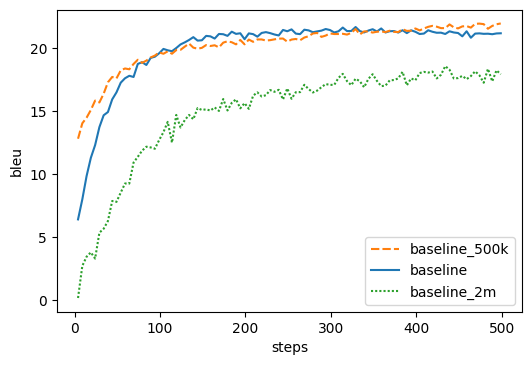
\includegraphics[width=0.85\textwidth]{img/baseline.png}}
    \centering
    \caption[Comparison between baseline models trained with different size of datasets.]{
        Comparison between baseline models trained with different size of datasets. \texttt{baseline} represents the model trained only using IWSLT; \texttt{baseline\_500k} represents the model trained using IWSLT and WMT with total of 500k sentence pairs; \texttt{baseline\_2m} represents the model trained using IWSLT and WMT with total of 2 million sentence pairs.}
    \label{img:basecomp}
\end{figure}

\subsubsection{Experiment Results}

In this section, we compare the result of the baseline models with the fine-tuned models with adapters. Our first experiment compared the results from an empty BERT model (a transformer model with BERT configuration but no pre-trained BERT weights) without any pre-training and adapters and only trained the model from scratch. We refer to these models as our \texttt{baseline} for the rest of this chapter. From \cref{img:basecomp}, we can see that adding more data to the baseline models does not necessarily improve the performance. We suspect the models require more training time to get the best final performance. There is a clear gap between \texttt{baseline\_2m} and the rest of the baseline models. \texttt{baseline} and \texttt{baseline\_500k} perform really well from the start while \texttt{baseline\_2m} lags behind. 
\hl{We recall from} \cref{ssec:langmodeldataset} \hl{that in the 2 million dataset we incorporate more sentence pairs by randomly sampling data from WMT19 and incorporating them onto IWSLT data, and due to this reason, there may be a distribution shift on the training data. Therefore, we suspect that the performance discrepancy is due to the aforementioned effect.} 
We found that \texttt{baseline\_500k} performs the best as it balances the models to avoid overfitting in the intended domain and still benefits from out-of-domain data. \texttt{baseline\_2m} shows the impact on domain difference where it has relatively lower performance than the other models. However, we must acknowledge that the model has not fully converged in the limited training time (measured by the number of steps) we have and has a chance to improve its performance further. Despite the lower performance in BLEU score, \texttt{baseline\_2m} deserves a manual evaluation of the translation output. We argue that in some cases, lower BLEU may not necessarily reflect a lower quality. We perform the manual evaluation at a later stage in this chapter.

To see the impact of adapters, we compare the result on different sizes of pre-training data used for the base model. The base models are then fine-tuned with the adapters module on the IWSLT data. As we can see from \cref{img:adpcomp}, pre-trained BERT with adapters achieves the best performance from the earlier steps compared to the rest of the models. In contrast to the baseline models, we see the benefit of adding more sentences to the pre-training (see \texttt{adapters\_pt\_2m} vs \texttt{adapters\_pt\_500k}). From \cref{img:basecomp} we see that \texttt{baseline\_500k} outperforms \texttt{baseline\_2m} by approximately 5 BLEU despite larger training data on \texttt{baseline\_2m}. Note that the training data we refer to in the baseline models is the training data for MT. On the other hand, when we add more training data on the pre-training side, we can see that the model trained using 500k data has a lower performance than the one using 2 million data. This tells us that adding larger pre-training monolingual data and then fine-tuning the models with adapters impact the performance positively.

\begin{figure}[h]
    {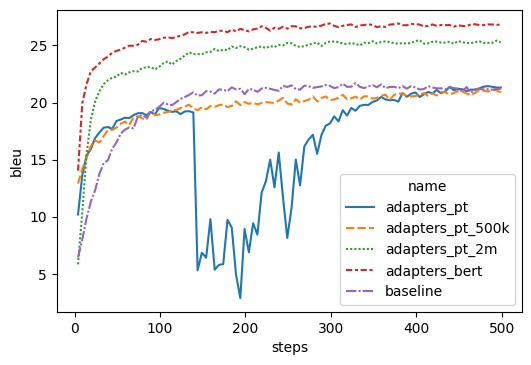
\includegraphics[width=0.75\textwidth]{img/adapterscomparison.png}}
    \centering
    \caption[The effect of pre-training data size when the adapters are then trained on the same IWSLT data.]{
        The effect of pre-training data size when the adapters are then trained on the same IWSLT data. \texttt{baseline} represents the model trained only using IWSLT; \texttt{adapters\_pt} represents the model pre-trained only using IWSLT; \texttt{adapters\_pt\_500k} represents the model pre-trained using IWSLT and WMT with total of 500k sentence pairs; \texttt{adapters\_pt\_2m} represents the model pre-trained using IWSLT and WMT with total of 2 million sentence pairs; \texttt{adapters\_bert} represents the model that uses BERT weights.}
    \label{img:adpcomp}
\end{figure}

In the model that only uses IWSLT as the pre-training data, we observe performance degradation in the middle of the fine-tuning. We found this is due to the gradient explosion in the cross-attention layer, and we attribute this instability to the small data used in the pre-training. In the later steps, the IWSLT model eventually achieved performance similar to the 500k model.

\subsection{Random and Shuffled Pre-trained Weights}
\label{ssec:randshuff}
\subsubsection{Experiment Setup and Motivation}
We perform two different categories of experiments to study how the adapters benefit from the pre-trained weights.
First, we conduct experiments where we shuffle the BERT weights. We separate the weights initialization into two approaches to perform the experiments:
\begin{itemize}
    \item We shuffled the weights from the column perspective. We shuffled the column-wise order of all the matrices while keeping the row-wise order intact.
    \item We shuffled the weights from both column and row perspectives.
\end{itemize}

Second, we conduct experiments where we set random weights on all base network layers and treat them as the pre-trained model. During the fine-tuning, we only update the adapter weights and keep the random weights intact.

\subsubsection{Experiment Results}
We can see from \cref{img:shfrndcmp} that the performance of the model that uses random pre-trained weights is more stable than the one using shuffled BERT weights. All shuffled BERT models suffer from gradient explosion similar to the IWSLT model we show in the previous section. Furthermore, shuffling the weights on both the row and column sides seems more detrimental than just shuffling on the column side. This may show that there could be some pattern in \texttt{adapters\_shuffled} that the adapters can eventually help to recover during the fine-tuning, while on \texttt{adapters\_shuffled\_both} more patterns are missing and more challenging to recover.

Although the performance of the random model (\texttt{adapters\_random}) is still below the baseline model, it is interesting to see that fine-tuning only the adapters, cross-attention, and output layers is sufficient to achieve a reasonable BLEU score, considering that the pre-trained model does not contain meaningful information relative to the original BERT weights. Furthermore, it is also interesting to see that compared to \texttt{adapters\_shuffled\_both}, we can get better final performance even though we can categorize \texttt{adapters\_shuffled\_both} as a model that uses randomly set weights pre-trained model. We hypothesize that this is probably related to the difference in the distribution of the weights between the models. In \texttt{adapters\_random} we are limited to the distribution of the weights in the initialization algorithm used in BERT, while in \texttt{adapters\_shuffled\_*} the distribution may be different as the weights in pre-trained BERT have already been optimized with the MLM objective.

\begin{figure}[h]
    {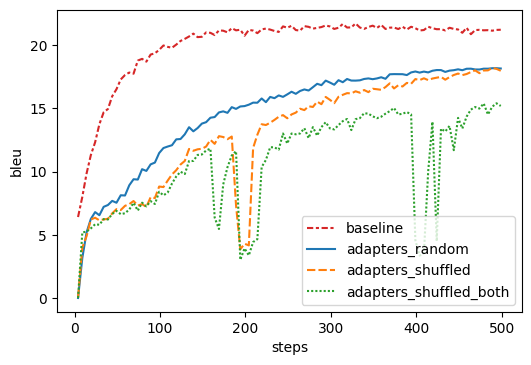
\includegraphics[width=0.85\textwidth]{img/randomshuffled.png}}
    \centering
    \caption[Comparison between adapters using shuffled BERT and random weights as the pre-trained models.]{Comparison between adapters using shuffled BERT and random weights as the pre-trained models. \texttt{baseline} represents the model trained only using IWSLT; \texttt{adapters\_random} represents the model pre-trained only using random weights; \texttt{adapters\_shuffled} represents the model pre-trained using column-wise shuffled BERT model; \texttt{adapters\_shuffled\_both} represents the model pre-trained using shuffled BERT model.}
    \label{img:shfrndcmp}
\end{figure}

Since we are relying on the pre-trained model with a random set of weights and with no further training, there is a possibility that our method may only work in a single random seed. To ensure a robust experiment, we repeat the random experiments ten times with ten different random seeds. We can see from the result in \cref{img:rndmseed} that all the random seed performs similarly to one another.

\begin{figure}[h]
    {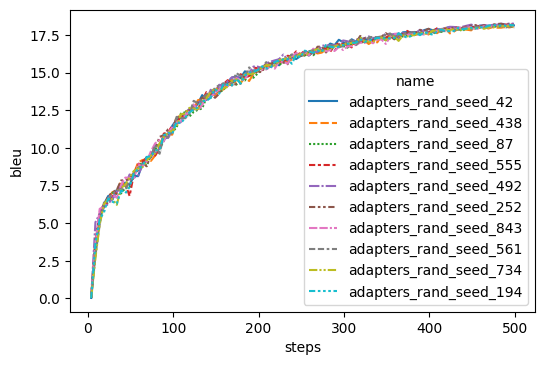
\includegraphics[width=0.85\textwidth]{img/adapter_random_multiseed.png}}
    \centering
    \caption{Comparison of different random seed for randomly set weights based models.}
    \label{img:rndmseed}
\end{figure}

\subsection{Random Pretrained vs. Out-of-Domain Data}
\label{ssec:randpre}
\subsubsection{Experiment Setup and Motivation}
In this experiment, we use the same setup as in \cref{ssec:adaptcomp,ssec:randshuff}. Specifically, we are interested in investigating the model's performance that uses randomly set weights as the pre-trained model compared to the baseline model. We recall that we can gain a reasonable score when fine-tuning the model with adapters from the previous experiments using randomly set pre-trained weights on the transformer model. In this experiment, we are conducting further study to understand the performance relative to the \texttt{baseline} model, where the model was trained using only IWSLT data and a different baseline (\texttt{baseline\_2m}), where the model was trained using a mix of WMT and IWSLT.
\newpage
This comparative study aims to understand whether we can see the benefits of using adapters versus training the whole transformer model with bigger data sizes.

\subsubsection{Experiment Results}

\begin{figure}[h]
    {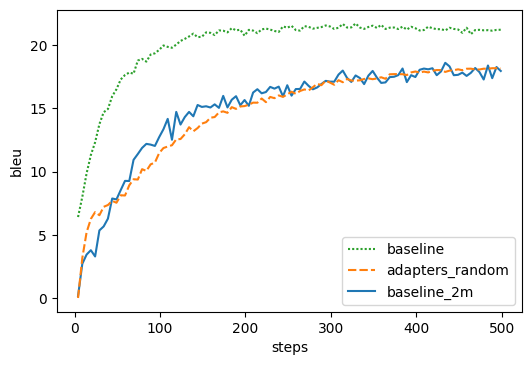
\includegraphics[width=0.85\textwidth]{img/random.png}}
    \centering
    \caption[Comparison between pre-trained random weights and baseline model.]{Comparison between pre-trained random weights and baseline model. \texttt{baseline} represents the model trained only using IWSLT; \texttt{baseline\_2m} represents the baseline model trained with a combination of IWSLT and WMT sentence pairs; \texttt{adapters\_random} represents the model pre-trained only using random weights.}
    \label{img:rndbslcmp}
\end{figure}

We analyze the random weights by comparing the result with the best-performing baseline and our pre-trained transformer models. From \cref{img:rndbslcmp}, we can see that the performance of the random model achieves a similar result as the baseline model that uses 2 million training sentence pairs. Recall that the baseline model is the BERT-style transformer model trained from scratch without fine-tuning and adapters. This tells us that training the whole model with bigger data does not necessarily improve the model's performance. It may need further tuning to gain the benefits of bigger data and bigger models because any departure from the domain of the test set can be more harmful than useful. We can see the result of using random weights as a potential alternative for training the model with small data such as IWSLT. While the performance is still far from the baseline (no adapters, full model training on IWSLT, i.e. in-domain data), this result shows that the base model's structure helps the adapter achieve a meaningful performance with a tiny portion of weights trained in the fine-tuning.

\begin{table*}[h]
    \centering
    \begin{tabular}{@{}l@{}}
        \toprule
        \multicolumn{1}{c}{\textbf{Random Weights + Adapters}}                                                                                                                                                                                                                                                                                                            \\ \midrule
        \begin{tabular}[c]{@{}l@{}}\textbf{Input}: wir tanzen im tempel und werden zu gott. \& quot ;\\ \textbf{Reference}: we dance in the temple and become god . \&quot;\\ \textbf{Hypothesis}: we \& apos ; re going to be able to become god. \& quot ;\end{tabular}                                                                                                 \\ \midrule
        \begin{tabular}[c]{@{}l@{}}\textbf{Input}: aber gleichzeitig hatten sie eine klare kenntnis des waldes, \\ die erstaunlich war.\\ \textbf{Reference}: but at the same time they had a perspicacious knowledge of the\\ forest that was astonishing.\\ \textbf{Hypothesis}: but at the same time, they had a clear of the audience\\ who was amazing.\end{tabular} \\ \midrule
        \begin{tabular}[c]{@{}l@{}}\textbf{Input}: es ist so wunderbar. ihr musst es beschutzen. \& quot ;\\ \textbf{Reference}: it is that beautiful . it is yours to protect . \&quot;\\ \textbf{Hypothesis}: it \& apos ; s wonderful. you have to protect it. \& quot ;\end{tabular}                                                                                  \\ \bottomrule
    \end{tabular}
    \caption{Prediction results from randomly set pre-trained model fine-tuned with adapters.}
    \label{tab:qtrand}
\end{table*}

We perform a quick check of the output of the model in \cref{tab:qtrand}. From the first two lines, we can see that the model has difficulty capturing complex phrases. In the first row, the model missed \textbf{tanzen im tempel} which means \textbf{dancing in the temple}. For the second row, the model confuses \textbf{knowledge of the forest} and outputs \textbf{audience} instead. Furthermore, the model also does not translate the word \textbf{kenntnis} and makes the translation unclear since the object of the sentence is missing. Despite those mistakes, the model still can capture simple sentences, as shown in the third row. Another observation that we noticed is the tokenization of \texttt{\&quot\;} and \texttt{\&amp\;}. Instead of being treated as a single token, the tokenizer splits them into three different subword tokens. We notice that this is due to the unavailability of the tokens in the pre-trained BERT vocabulary.

\section{Qualitative Comparison}
\begin{sidewaystable*}
    \centering
    % \begin{tabular}{|l|l|l|}
    %     \hline
    %     \multicolumn{1}{|c|}{\textbf{Baseline IWSLT}}                                                                                                                                                                                                                     &
    %     \multicolumn{1}{c|}{\textbf{IWSLT + WMT (total 2m)}}                                                                                                                                                                                                              &
    %     \multicolumn{1}{c|}{\textbf{BERT + Adapters}}                                                                                                                                                                                                                                \\ \hline
    %     \begin{tabular}[c]{@{}l@{}}\textbf{input}: erinnerst du dich an\\ den patienten\\ mit dem gereizten rachen? \\ \textbf{prediction}: do you remember\\ reading to the patients? on the\end{tabular}                                                                &
    %     \begin{tabular}[c]{@{}l@{}}\textbf{input}: erinnerst du dich an\\ den patienten\\ mit dem gereizten rachen? \\ \textbf{prediction}: do you remember\\ the patient with the tingling\\ revenge?\end{tabular}                                                       &
    %     \begin{tabular}[c]{@{}l@{}}\textbf{input}: erinnerst du dich an\\ den patienten\\ mit dem gereizten rachen? \\ \textbf{prediction}: remember the\\ patient with\\ the bruised remorse?\end{tabular}                                                                          \\ \hline
    %     \begin{tabular}[c]{@{}l@{}}\textbf{input}: großartig, sagte ich.\\ legte auf.\\ \textbf{prediction}: great, i said.\\ got up..\end{tabular}                                                                                                                       &
    %     \begin{tabular}[c]{@{}l@{}}\textbf{input}: großartig, sagte ich.\\ legte auf.\\ \textbf{prediction}: great, i said.\\ put on..\end{tabular}                                                                                                                       &
    %     \begin{tabular}[c]{@{}l@{}}\textbf{input}: großartig, sagte ich.\\ legte auf.\\ \textbf{prediction}: great, i said.\\ put it down.\end{tabular}                                                                                                                              \\ \hline
    %     \begin{tabular}[c]{@{}l@{}}\textbf{input}: - - aber in unserer\\ entdeckung der welt, haben\\ wir alle arten unterschiedlicher\\ methoden.\\ \textbf{prediction}: but in our discovery\\ of the world, we \& apos ;\\ ve got all sorts of different\end{tabular}  &
    %     \begin{tabular}[c]{@{}l@{}}\textbf{input}: - - aber in unserer\\ entdeckung der welt, haben\\ wir alle arten unterschiedlicher\\ methoden.\\ \textbf{prediction}: - - but in our discovery\\ of the world, we have\\ all kinds of different methods.\end{tabular} &
    %     \begin{tabular}[c]{@{}l@{}}\textbf{input}: - - aber in unserer\\ entdeckung der welt, haben\\ wir alle arten unterschiedlicher\\ methoden.\\ \textbf{prediction}: but in our discovery\\ of the world, we have\\ all sorts of different ways of doing\\ things.\end{tabular} \\ \hline
    % \end{tabular}
    % \begin{table}[]
    \begin{tabular}{@{}l@{}}
        \toprule
        \multicolumn{1}{c}{\textbf{Sample Translation Output}}                                                                                                                                                                                                                                                                                                                                                                                                                                                                                                                            \\ \midrule
        \begin{tabular}[c]{@{}l@{}}\textbf{Input}: erinnerst du dich an den patienten mit dem gereizten rachen?\\ \textbf{Reference}: do you remember that patient you saw with the sore throat?\\ \textbf{Hypothesis 1}: do you remember reading to the patients? on the\\ \textbf{Hypothesis 2}: do you remember the patient with the tingling revenge?\\ \textbf{Hypothesis 3}: remember the patient with the bruised remorse?\end{tabular}                                                                                                                                            \\ \midrule
        \begin{tabular}[c]{@{}l@{}}\textbf{Input}: großartig, sagte ich. legte auf.\\ \textbf{Reference}: great, i said. got off the phone.\\ \textbf{Hypothesis 1}: great, i said. got up..\\ \textbf{Hypothesis 2}: great, i said. put on..\\ \textbf{Hypothesis 3}: great, i said. put it down.\end{tabular}                                                                                                                                                                                                                                                                           \\ \midrule
        \begin{tabular}[c]{@{}l@{}}\textbf{Input}: - - aber in unserer entdeckung der welt, haben wir alle arten unterschiedlicher methoden.\\ \textbf{Reference}: but in our discovery around the world, we have all kinds of other methods.\\ \textbf{Hypothesis 1}: but in our discovery of the world, we \& apos ; ve got all sorts of different\\ \textbf{Hypothesis 2}: - - but in our discovery of the world, we have all kinds of different methods\\ \textbf{Hypothesis 3}: but in our discovery of the world, we have all sorts of different ways of doing things.\end{tabular} \\ \bottomrule
    \end{tabular}
    % \end{table}
    \caption{Prediction results from \textbf{Hypothesis 1}: Baseline model trained with only IWSLT data; \textbf{Hypothesis 2}: Pre-trained model with adapters where we pre-train the model with IWSLT and WMT with a total of 2 million pre-training data; \textbf{Hypothesis 3}: BERT with adapters.}
    \label{tab:qtvout}
\end{sidewaystable*}
% We perform a manual check to compare the generated results on some of our models.
We perform a manual check on the generated translations of some of our models.
From \cref{tab:qtvout}, we can see that none of the models generated the correct result for the first example. However, BERT + adapters and 2 million pre-trained base models generate the proper context where the result is still discussing \textbf{the patient}. The wrong part is when the model generates an incorrect translation regarding the patient's disease. The second example shows that the BERT + adapters model creates a better quality of translation than the other models. The final example shows that BERT + adapters generate an interesting output where it manages to remove unimportant characters such as ``\texttt{--}'' and produce readable output. People may vary in their opinion on this example as the 2 million pre-trained base model generates a more concise output.

We also notice that the BERT-based models have difficulties generating long sentences. The models always cut the translation short when an unavailable token such as \texttt{\&quot\;} appears in the sentence. To give a more explicit example, \cref{tab:errout} illustrates the significant difference in the outputs when the token \texttt{\&quot\;} is observed in the input. This shows that tokenization plays an essential role in the model where tokens unavailable in the vocabulary list may affect the generated output significantly.

\begin{table}[]
    \begin{tabular}{@{}l|l@{}}
        \toprule
        \multicolumn{1}{c}{\textbf{Input}}                                                                                                                                                          &
        \multicolumn{1}{c}{\textbf{Output}}                                                                                                                                                           \\ \midrule

        \begin{tabular}[c]{@{}l@{}}\& quot ; moneyball \& quot ; erscheint\\ bald und dreht sich um\\ statistiken und um diese zu nutzen\\ ein großartiges baseball team aufzustellen.\end{tabular} &
        \begin{tabular}[c]{@{}l@{}}\& quot ; devilball \& quot ; appears\\ soon, and it \& apos ;\end{tabular}                                                                                        \\ \midrule
        \begin{tabular}[c]{@{}l@{}}moneyball erscheint bald\\ und dreht sich um\\ statistiken und um diese zu\\ nutzen ein großartiges baseball\\ team aufzustellen.\end{tabular}                   &
        \begin{tabular}[c]{@{}l@{}}fatball soon appears and it\\ turns out statistics and\\ to use that to build a\\ great baseball team\end{tabular}                                                 \\ \bottomrule
    \end{tabular}
    \caption[An example of bad model behaviour when the input contains unknown tokens.]{An example of bad model behaviour when the input contains unknown tokens like \texttt{\&quot\;} (top row). The translation is not abruptly cut if these symbols are removed (bottom row).}
    \label{tab:errout}
\end{table}